\noindent \textred{1.} 
Consider the following graph, with node 0 as the source node.
\begin{figure}[!h]
    \centering
    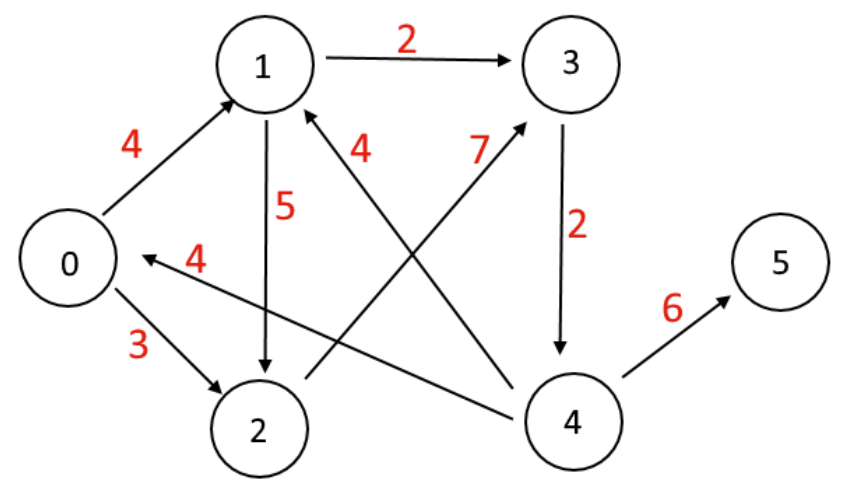
\includegraphics[width=0.5\linewidth]{HWs//HW12//figures/1.png}
\end{figure}
\begin{itemize}
    \item[(a)] Run Dijkstra’s algorithm. Write down the $d$ array before each EXTRACT-MIN, also the final array. 
    \begin{table}[!h]
        \centering
        \myAnswer{
        \begin{tabular}{c|ccccccc}
            \multirow{2}{*}{iteration $i$} & \multicolumn{7}{c}{$d$ array (before iteration $i$)} \\
            \cline{2-8}
             & index & 0 & 1 & 2 & 3 & 4 & 5 \\
            \hline
            1 &  & \textred{0} & $\infty$ & $\infty$ & $\infty$ & $\infty$ & $\infty$ \\
            2 &  & 0 & 4 & \textred{3} & $\infty$ & $\infty$ & $\infty$ \\
            3 &  & 0 & \textred{4} & 3 & 10 & $\infty$ & $\infty$ \\
            4 &  & 0 & 4 & 3 & \textred{6} & $\infty$ & $\infty$ \\
            5 &  & 0 & 4 & 3 & 6 & \textred{8} & $\infty$ \\
            6 &  & 0 & 4 & 3 & 6 & 8 & \textred{14} \\
        \end{tabular}
        }
    \end{table}
    \item[(b)] Run Bellman-Ford algorithm. Write down the $d$ distance array after each pass.
    \begin{table}[!h]
        \centering
        \myAnswer{
        \begin{tabular}{c|ccccccc}
            \multirow{2}{*}{vertex index } & \multicolumn{7}{c}{$d$ array (after pass $i$)} \\
            \cline{2-8}
             & index & 0 & 1 & 2 & 3 & 4 & 5 \\
            \hline
            1 &  & {0} & $\infty$ & $\infty$ & $\infty$ & $\infty$ & $\infty$ \\
            2 &  & 0 & 4 & {3} & $\infty$ & $\infty$ & $\infty$ \\
            3 &  & 0 & {4} & 3 & 6 & $\infty$ & $\infty$ \\
            4 &  & 0 & 4 & 3 & 6 & {8} & $\infty$ \\
            5 &  & 0 & 4 & 3 & 6 & 8 & {14} \\
        \end{tabular}
        }
    \end{table}

\end{itemize}
